\documentclass[12pt]{article}

%% Basic document formatting
\usepackage{amsmath, amsthm, amssymb, amsfonts}
\usepackage{mathtools}
\usepackage{mathrsfs}
\usepackage{xspace}
\usepackage{thmtools}
\usepackage{graphicx}
\usepackage{tikz-cd}
\usepackage{color}
\usepackage{setspace}
\usepackage{fancyhdr}
\usepackage{titling}
\usepackage{hyperref}
\usepackage[left=0.4in,right=0.4in,top=1in,bottom=1in]{geometry}
\usepackage{float}
\usepackage{tabularx}
\usepackage{booktabs}
\usepackage[utf8]{inputenc}
\usepackage[english]{babel}
\usepackage{framed}
\usepackage[dvipsnames]{xcolor}
\usepackage{environ}
\usepackage{tcolorbox}
\tcbuselibrary{theorems,skins,breakable}

\usepackage{enumitem}
\setlist[enumerate]{leftmargin=*}
\setlist[enumerate,1]{labelindent=\parindent}
\setlist[enumerate,2]{labelindent=0pt}

% Blackboard Bold
\newcommand{\Z}{\mathbb{Z}}                 % integers
\newcommand{\Zpl}{\mathbb{Z}_{+}}           % positive integers
\newcommand{\Znn}{\mathbb{Z}_{\geq 0}}      % nonnegative integers. 
\newcommand{\Q}{\mathbb{Q}}                 % rationals
\newcommand{\Qpl}{\mathbb{Q}_{+}}           % positive Rationals
\newcommand{\R}{\mathbb{R}}                 % reals
\newcommand{\Rpl}{\mathbb{R}_{+}}           % positive Reals
\newcommand{\C}{\mathbb{C}}                 % complex numbers
\newcommand{\F}{\mathbb{F}}                 % field

% Words
\newcommand{\st}{\text{ such that }}
\newcommand{\wrt}{\text{ with respect to }}
\newcommand{\with}{\text{ with }}
\newcommand{\ie}{\text{, i.e. }}
\newcommand*{\ditto}{\text{---}\texttt{"}\text{---}}

% Operators
\newcommand{\abs}[1]{\left|#1\right|}                   % absolute value
\newcommand{\norm}[1]{\abs{\abs{#1}}}
\newcommand{\floor}[1]{\left\lfloor #1 \right\rfloor}   % floor
\newcommand{\ceil}[1]{\left\lceil #1 \right\rceil}      % ceiling
\newcommand{\powset}[1]{\mathscr{P}(#1)}

% Category Theory 
\renewcommand{\hom}{\text{Hom}}
\newcommand{\homspace}[3]{\hom_{#1}(#2, #3)}
\newcommand{\coproduct}[9]{
  \begin{tikzcd}[ampersand replacement=\&]
      \& \& #1 \arrow[dll, bend right, "#6"] \arrow[dl, "#5"] \\
   #4 \& #3 \arrow[l, "#9"] \\
      \& \& #2 \arrow[ull, bend left, "#8"] \arrow[ul, "#7"]
  \end{tikzcd}
}

\newcommand{\product}[9]{ 
  \begin{tikzcd}[ampersand replacement=\&]
      \& \& #3 \\
      #1 \arrow[r, "#7"] \arrow[urr, bend left, "#5"] \arrow[drr, bend right, "#6"] \& #2 \arrow[ur, "#8"] \arrow[dr, "#9"] \\ 
      \& \& #4
  \end{tikzcd}
}


% Algebra 
\newcommand{\Syl}[2]{\text{Syl}_{#1}{(#2)}}           % set of Sylow-p subgroups 
\newcommand{\<}{\langle}                % \<x\>, subgroup generated by x 
\renewcommand{\>}{\rangle}
\renewcommand{\index}[2]{[#1 : #2]}
\newcommand{\id}{\text{id}}             % identity element
\newcommand{\lhdneq}{%
  \mathrel{\ooalign{$\lneq$\cr\raise.22ex\hbox{$\lhd$}\cr}}}
\newcommand{\order}[1]{\text{o}(#1)}    % order of an element
\newcommand{\spec}{\operatorname{Spec}}
\newcommand{\rad}{\operatorname{rad}}   % radical of an ideal 
\newcommand{\sym}[1]{\mathfrak{S}_{#1}}
\newcommand{\aut}[1]{\text{Aut}(#1)} 
\newcommand{\gal}[2]{\text{Gal}(#1 / #2)} 
\newcommand{\inn}[1]{\text{Inn}(#1)} 
\let\oldcong\cong
\let\oldequiv\equiv
\renewcommand{\cong}{\oldequiv}
\renewcommand{\equiv}{\oldcong}

\newcommand{\triangleleftneq}{\mathrel{\ooalign{%
  $\trianglelefteq$\cr
  \hidewidth\raise0.06ex\hbox{$\not\mkern4mu$}\hidewidth\cr
}}}

\makeatletter % cycle
\newcommand{\cyc}[1]{(\mathbf{\cyc@process#1\relax})}
\def\cyc@process#1#2\relax{%
	#1%
	\ifx\relax#2\relax
	\else
		\,\cyc@process#2\relax
	\fi
}
\makeatother

\newcommand{\GL}[2]{\text{GL}_{#1}(#2)}                             % general linear group
\newcommand{\SL}[2]{\text{SL}_{#1}(#2)}                             % special linear group
\newcommand{\gl}[2]{\mathfrak{gl}_{#1}(#2)}
\renewcommand{\sl}[2]{\mathfrak{sl}_{#1}(#2)}
\newcommand{\so}[2]{\mathfrak{so}_{#1}(#2)}
\newcommand{\su}[1]{\mathfrak{su}(#1)}

% Linear Algebra
\newcommand{\bmat}[1]{\begin{bmatrix}#1\end{bmatrix}}   % bracketed matrix
\newcommand{\rank}{\operatorname{rank}}                 % rank
\newcommand{\nullity}{\operatorname{nullity}}           % nullity
\newcommand{\tr}{\operatorname{tr}}

% Combinatorics
\newcommand{\qnum}[1]{\left[#1\right]_q}                % q-analog
\newcommand{\qfact}[1]{\left[#1\right]!_q}              % q-analog factorial 
\newcommand{\qbinom}[2]{\binom{#1}{#2}_q}               % Gaussian binomial coefficient

% Topology/Analysis
\newcommand{\ball}[2]{\text{B}_{#1}(#2)}  % B_r(x): open r-balls around x
\newcommand{\diam}{\text{diam}}           % diamter of a set in metric space 
\newcommand{\lowint}[2]{\underline{\int_{#1}^{#2}}}
\newcommand{\upint}[2]{\overline{\int}_{#1}^{#2}}

% Misc Notation
\newcommand{\oneton}[1]{\{1, \ldots, #1\}}
\newcommand{\defeq}{\vcentcolon=}   % :=
\newcommand{\eqdef}{=\vcentcolon}   % =: 
\renewcommand{\bf}[1]{\textbf{#1}}
\newcommand{\im}{\operatorname{im}}
\newcommand{\fnrest}[2]{\left.#1\right|_{#2}}
\newcommand{\isom}{\overset{\sim}{\rightarrow}} 


\renewcommand{\thesection}{\arabic{section}.}
\renewcommand{\thesubsection}{(\alph{subsection})}

\newtheorem{claim}{Claim}
\newtheorem*{lemma}{Lemma}

%% Headers & title setup
\newcommand{\course}{Math100C}
\newcommand{\myname}{Jay Ser}
\setlength{\headheight}{14.5pt}
\pagestyle{fancy}
\fancyhf{}
\renewcommand{\headrulewidth}{0.4pt}
\lhead{\course}
\rhead{\myname}
\cfoot{\thepage}
\setlength{\droptitle}{-4em} 
\title{\course\ - WK9} 
\author{\myname}
\date{2026.05.31}

\begin{document}
\maketitle
\thispagestyle{fancy}


%------------------------------------------------------------------------------%

\section{} 
Determine the Galois group of the splitting field of the minimal polynomials of the following quantities: 
$$\sqrt{5 + \sqrt{13}},\quad \sqrt{5 + \sqrt{21}},\quad \sqrt[3]{2 + \sqrt{2}}, \quad \sqrt[3]{2 + \sqrt[3]{2}}$$

\noindent \dotfill 

I need so much help! 

\section{} 

\subsection{}

Show that for any prime $p$, 
$$\sum_{j = 0}^{p - 1} e^{2\pi i j^2 / p}$$ 
is a square root of either $p$ or $-p$. 
Then deduce that every quadratic extension of $\Q$ is contained in $Q(\zeta_n)$ for some positive integer $n$. 

\noindent \dotfill 

Let 
$$\chi(k) = \begin{cases} 
  1 & \text{if } k \text{ is a square } \mod p \\ 
  -1 & \text{else} 
\end{cases}$$
be the Legendre symbol (recall that the Legendre symbol is a homomorphism). 
For brevity, let $\zeta$ be the primitive $p$th root of unity. 
\begin{align}
  \sum_{j = 0}^{p - 1} e^{2\pi i j^2 / p} 
  & = 1 + \sum_{j \in \F_p^{\times}} \zeta^{j^2 \mod p} \nonumber \\ 
  & = 1 + \sum_{k \in \F_p^{\times}} (1 + \chi(k)) \zeta^k  \label{eq:2_legendre} \\ 
  & = 1 + \sum_{k \in \F_p^{\times}} \zeta^k + \sum_{k \in \F_p^{\times}} \chi(k) \zeta^k \nonumber \\ 
  & = \sum_{k \in \F_p^{\times}} \chi(k) \zeta^k \label{eq:2_res1} 
\end{align}
where \eqref{eq:2_legendre} follows because if $k \in \F_p$ is a square mod $p$, i.e., $x^2 - k$ has at least one solution in $\F_p$, then in fact $x^2 - k$ has exactly two solutions. 
Following on from \eqref{eq:2_res1}, 
\newcommand{\field}{\F_p^{\times}}  
\begin{align}
  (\sum_{j = 0}^{p - 1} e^{2\pi i j^2 / p})^{2} 
  & = \sum_{a \in \field}\sum_{b \in \field} \chi(a) \chi(b) \zeta^{a + b}  \nonumber = \sum_{a \in \field} \sum_{b \in \field} \chi(ab) \zeta^{a + b}  \nonumber \\ 
  & = \sum_{a \in \field} \sum_{b \in \field} \chi(a ab) \zeta^{a + ab}, \label{eq:2_sub}  \\ 
  & = \sum_{a \in \field} \sum_{b \in \field} \chi(b) \zeta^{a(1 + b)} \nonumber = \sum_{b \in \field} \chi(b) \sum_{a \in \field} \zeta^{a(1 + b)} \nonumber \\ 
  & = \sum_{\substack{b \in \field \\ b = -1}} \chi(-1) \sum_{a \in \field} \zeta^{0} + \sum_{\substack{b \in \field \\ b \neq -1}} \chi(b) \sum_{a \in \field} \zeta^{a(1 + b)} \nonumber \\ 
  & = (p - 1)\chi(-1) + \sum_{\substack{b \in \field \\ b \neq -1}} \chi(b) \sum_{a \in \field} \zeta^{a} \label{eq:2_sub2} \\ 
  & = (p - 1)\chi(-1) - \sum_{\substack{b \in \field\\ b \neq -1}} \chi(b) \nonumber \\ 
  & = (p - 1)\chi(-1) + \chi(-1) = p\chi(-1) \nonumber
\end{align}
where \eqref{eq:2_sub} follows from the substitution $b \mapsto ab$ and the fact that $ab$ and $b$ permute over the same elements in the group $\field$; 
similarly, \eqref{eq:2_sub2} follows from the substitution $a \mapsto a(1 + b)^{-1}$ in $\F_p^{\times}$, where $(1 + b)^{-1}$ is guaranteed to exist when summing over $b \in \F_p^\times \setminus \{-1\}$. 
The equality 
$$ (\sum_{j = 0}^{p - 1} e^{2\pi i j^2 / p})^{2} = p\chi(-1)$$ 
shows that $(\sum_{j = 0}^{p - 1} e^{2\pi i j^2 / p})^{2}$ is indeed a square root of $p$ or $-p$. 

\subsection{}
Show every quadratic extension of $\Q$ is contained in some $\Q(\zeta_n)$. 

\noindent \dotfill 

All quadratic extensions of $\Q$ are of the form $\Q(\sqrt{d})$ for a square-free integer $d$. 
Write $d = p_1 \cdots p_k$ with each prime factor distinct. 
By subsection (a), 
$$\sqrt{d} \in \Q(\zeta_{p_1}, \ldots, \zeta_{p_k}, i) = \Q(\zeta_n)$$ 
where $i = \sqrt{-1}$ is thrown in since, a priori, it's unclear if which of $\sqrt{+d}$ or $\sqrt{-d}$ is inside $\Q(\zeta_{p_1}, \ldots, \zeta_{p_k})$. 
This shows $\Q(\sqrt{d}) \subset \Q(\zeta_n)$. 

\section{} 
Let $f(x) = x^5 - 3x + 1$. 
\subsection{}
Show $f$ is irreducible over $\Q$. 

\noindent \dotfill


By the rational root theorem or whatever, only possible roots of $f$ are $\pm 1$; 
clearly neither are roots, so $f$ has no linear factor. 
Suppose $f(x) = (x^2 + ax \pm 1)(x^3 + bx^2 + cx \pm 1)$. 
In the $+1$ case, one can solve the linear system to get 
$$c - (3 + c)^2 + 1 = 0,$$
which has no solutions over $\R$ (and thereby $\Q$). 
Similarly, in the $-1$ case, one obtains 
$$3 - a - a^2 = 0$$
but $a$ cannot be rational since $3 - x - x^2$ is irreducible over $\Q$ by the rational root test. 
Hence $f$ cannot have a quadratic root either; 
$f$ is irreducible over $\Q$. 

\subsection{} 
Verify using some computer system to show $f(x)$ has exactly three roots. 

\noindent \dotfill 

Graph the function on desmos! 
The three real roots of $f$ are around $-1.4$, $0.3$, and $1.2$. 

\subsection{} 
Deduce that the Galois group of $f$ is $\sym{5}$. 

\noindent \dotfill 

Since $f$ has complex roots (which must be conjugates), the Galois group of $f$ contains a transposition; 
namely, the automorphism that swaps the complex roots and is identity on all other elements. 
Further, since $f$ is irreducible, the Galois group contains a 5-cycle. 
Hence the Galois group of $f$ is $\sym{5}$. 

\section{} 
Find a degree 7 polynomial whose Galois group is $\sym{7}$. 

\noindent \dotfill 

$$f(x) = x^7 = 8x^6 -12x^4 + 2$$
satisfies the desired property. 
It is irreducible by Eisenstein for $p = 2$, and it has five real roots: 
\begin{center}
  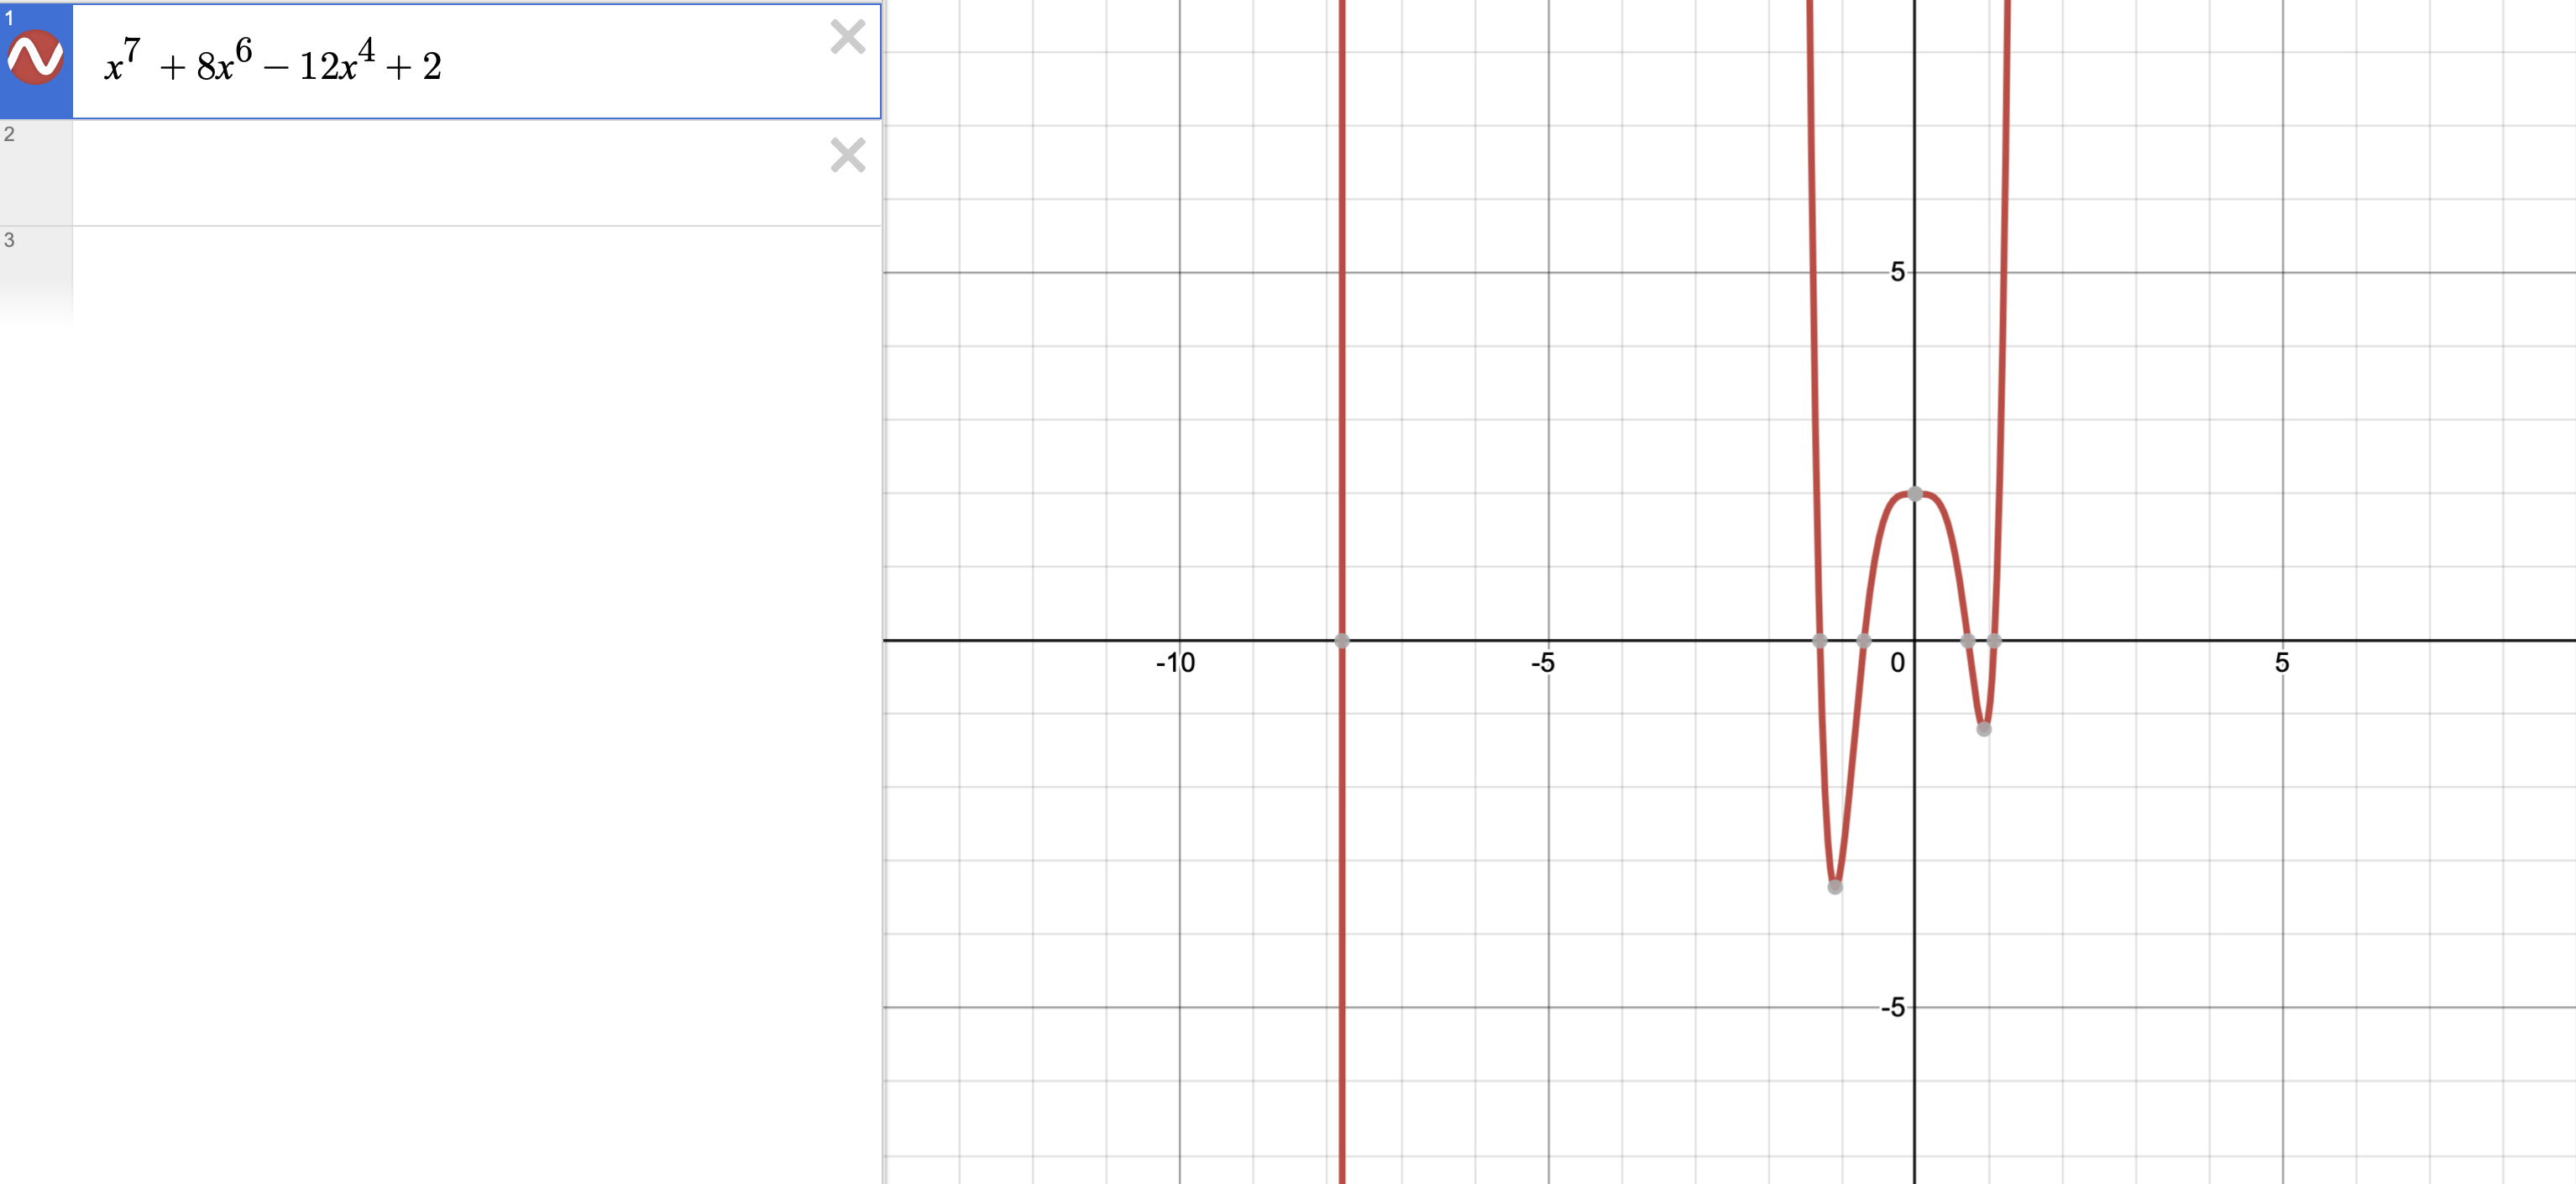
\includegraphics[scale=0.3]{./img/deg7.png}
\end{center}
By the same process as Q3, the Galois group of $f$ is $\sym{7}$. 

\section{} 
Let $K / F$ be a Galois extension. 
Determine the number of subfields of $K$ of each possible degree over $F$ in each of the following cases: 
$$\gal{K}{F} \equiv D_4, \quad \gal{K}{F} \equiv A_4$$

\noindent \dotfill 

\subsection{} 
Let $D_4 = \<x, y \mid x^4 = y^2 = 1; \, yx = x^3 y\>$. 
The diagram below is the lattice for $D_4$: 
it contains two copies of the Klein Four group, one 4-cycle, and five 2-cycles. 

\begin{center}
\begin{tikzcd}
  & & D_4 \arrow[d, no head] \arrow[dr, no head] \arrow[dl, no head] \\
  & \<x^2, y\> \arrow[d, no head] \arrow[dr, no head] \arrow[dl, no head] & \<x\> \arrow[d, no head] \arrow[dr, no head] \arrow[dl, no head] & \<x^2, xy\>  \arrow[d, no head] \arrow[dr, no head] \arrow[dl, no head] \\
  \<y\> & \<x^2 y \> & \<x^2\> & \<xy\> & \<x^3 y\> \\
		&  & 1 \arrow[ull, no head] \arrow[ul, no head] \arrow[u, no head] \arrow[ur, no head] \arrow[urr, no head] 
\end{tikzcd} 
\end{center}

Accordingly, by the main theorem of Galois theory, the subfields of $K$ over $F$ are: 
\begin{itemize}
  \item One degree 8 extension, namely $K$ itself
  \item Five degree 4 extensions corresponding to the 2-cycles
  \item Three degree 2 extensions corresponding to the Klein Four groups 
  \item One degree 1 extension, $F$ itself
\end{itemize}

\subsection{} 
\begin{center}
\begin{tikzcd} 
  & & & A_4 \arrow[dll, no head] \arrow[dd, no head] \arrow[ddr, no head] \arrow[ddrr, no head] \arrow[ddrrr, no head]  \\
  & V_4 \arrow[ddl, no head] \arrow[dd, no head] \arrow[ddr, no head]  \\ 
  & & & \<(123)\> & \<(124)\> & \<(134)\> & \<(234)\>  \\ 
  \<(12)(34)\> & \<(13)(24)\> & \<(14)(23)\>  \\ 
			   & & & 1 \arrow[ulll, no head] \arrow[ull, no head] \arrow[ul, no head] \arrow[uu, no head] \arrow[uur, no head] \arrow[uurr, no head] \arrow[uurrr, no head]  \\ 
\end{tikzcd} 
\end{center}
The above is the lattice for $A_4$: 
clearly its order 2 and order 3 groups are generated by the double transpositions and three-cycles. 
Since there are only three nonidentity elements of $A_4$ (double transpositions) with order dividing 4, the only possible order four subgroup would be the set containing the identity and al the double transpositions, and it turns out this is the Klein Four group. 
The only other possible subgroup of $A_4$ is a subgroup of order 6, but not such subgroup exists: any subset of $A_4$ with six elements has at least one three-cycle and a double transposition, but then a subgroup generated by a three-cycle and a double-transposition is the entire $A_4$. 

Accordingly, by the main theorem of Galois theory, the subfields of $K$ over $F$ are: 
\begin{itemize}
  \item One degree 12 extension, $K$ itself
  \item Three degree 6 extension, corresponding to the two-cycles
  \item Four degree 4 extensions, corresponding to the three-cycles
  \item One degree 3 extension, corresponding to $V_4$
  \item One degree 1 extension, $F$ itself 
\end{itemize}

\section{} 
Show that $A_6$ is simple. 

\noindent\dotfill 

I saw this proof in Rotman's \textit{An Introduction to the Theory of Groups}. 
Take a nontrivial normal subgroup $H \lhd A_6$ and a nontrivial element $h \in H$. 
Consider the case that some index $k$ is fixed by $h$. 
Letting 
$$K = \{a \in A_6 \mid a(i) = i\},$$
$K$ can be identified as $A_5$ since it consists of even permutations of $6 - 1 = 5$ indices. 
$h \in H \cap K$, so namely $H \cap K$ is nontrivial. 
But clearly $H \cap K \lhd K$; 
$A_5$ is simple, so one concludes $H \cap K = K$, i.e., $K \subset H$. 
$K$ contains a three-cycle of $A_5$, so $H$ contains a three-cycle, say $(123)$.
But all three-cycles are conjugate in $A_6$: 
take another three-cycle $(xyz)$. 
A permutation $\sigma \in \sym{6}$ sending 
$$1 \mapsto x, \quad 2 \mapsto y, \quad 3 \mapsto z$$ 
satisfies $\sigma (123) \sigma^{-1} = (abc)$. 
Namely, $\sigma$ can be taken to be even: 
if some $\sigma$ mapping as above is odd, then multiply $\sigma$ by $(45)$. 
Then conjugating $(123)$ by $\sigma (45)$, an even permutation, still yields $(xyz)$. 
Hence $H$ contains all the 3-cycles, and the 3-cycles generate $A_6$. 
Hence $H = A_6$. 

In other words, if $H \lhd A_6$ contains any element that fixes at least one index, then $H = A_6$. 
Next, consider the case that no element of $H$ fixes any index. 
After relabeling, the elements of $\sym{6}$ that achieve this are of the form 
$$(12)(34)(56), \quad (12)(3456), \quad (123)(456)$$
but only the latter two are even permutations. 
So all nonidentity elements of $H$ are of those two cycle types. 
But the second power of $(12)(3456)$ is a four cycle that fixes 1 and 2. 
Meanwhile, since $H$ is normal in $A_5$, if $H$ contains $(123)(456)$, then it contains 
$$(234) (123)(456) (243) = (14)(265)$$
which is an odd permutation, a contradiction. 
This shows that the only normal, nontrivial subgroup of $A_6$ is $A_6$ itself. 

\section{} 
Show that every Galois extension of degree 10 is solvable. 

\noindent \dotfill 

Let $G$ be the Galois group of a degree 10 Galois extension. 
Notice $10 = 2 \cdot 5$ is a group of order $pq$ with $q \mid (p - 1)$. 
By the Sylow theorems, there are two isomorphism classes for $G$: 
$G \equiv Z_2 \times Z_5 \equiv Z_{10}$, the cyclic group of order 10, or $G \equiv Z_2 \rtimes Z_5 \equiv D_5$, the dihedral group of a pentagon. 
Any abelian group is solvable, and the chain of subgroups of $D_5 = \<x, y \mid x^5 = y^2 = 1; \, yx = x^4 y\>$ 
$$1 < \<x\> < D_5,$$
with the identification $D_5 / \<x\> \equiv \<y\> \equiv Z_2$, shows $D_5$ is a solvable group. 
Hence any Galois extension of degree 10 is solvable. 

\section{} 
\subsection{} 
I follow the derivation given by Kiran. 
Let $f = x^p - a$ and $\zeta$ be the primitive $p$th root of unity. 
Let $K$ be the splitting field for $f$ over $F$. 
The quotient of the roots of $f$ is a $p$th root of unity, so $F(\zeta) \subset K$. 

First, assume this inclusion is proper. 
By Kummer's theorem, the intermediate extension $K / F(\zeta)$ is cyclic of degree $p$. 
But then the Galois group of this intermediate extension is a $p$-cycle on the roots of $f$, i.e., it is transitive on the roots of $f$. 
This shows $f$ is irreducible. 

It follows that if $f$ factors, then $F(\zeta) = K$. 
The Galois group of a Galois cyclotomic extension is a subgroup of $(\Z / p\Z)^\times$. 
Call the Galois group $G = \<c\> \subset (\Z / p\Z)^\times$; 
it has order $d$ dividing $p - 1$. 
Viewing $c$ as both the number generating $(\Z / pZ)^\times$ and the automorphism generating the Galois group, 
$$c: \zeta \mapsto \zeta^{c}$$
If $c = 1$, then the Galois group is trivial; 
$K = F$ and $f$ splits in $F$, and there is nothing more to show. 
Suppose $c \neq 1$. 
Take $\beta$ to be an arbitrary root of $f$. 
$$c: \beta \mapsto \zeta^k \beta,$$
for some $k \in \Z/p\Z$, so the orbit of $\beta$ under the action of $G = \<c\>$ is 
\begin{equation} \label{eq:8_orbit} 
  \beta, \zeta^k \beta, \zeta^{ck + k} \beta, \zeta^{c^2 k + ck + k} \beta, \ldots,
\end{equation}
where the elements eventually cycle. 
If $k = 0$, then the orbit is just $\beta$ and $\beta \in F$ since $\beta$ is fixed by every element of $G$. 
Suppose $k \neq 0$. 
Disregarding the factor $k$, notice that exponents of $\zeta$ are 
$$0, 1, c + 1, (c^2 + c + 1), \ldots$$
i.e., of the form $(c^t - 1)/(c - 1)$. 
By definition of $G = \<c\>$, $c$ has order $d$ in $(\Z / p\Z)^\times$, so that general term has form $(c^t - 1)(c - 1)$ shows the cycle above has period $d$, 
i.e., \eqref{eq:8_orbit} has $d$ distinct elements. 

The paragraph above shows that in the case $K = F(\zeta)$ with $\index{K}{F} = d$, the orbits of the roots under the action of the Galois group has sizes 1 or $d$. 
Suppose $d > 1$ and none of the orbits of the roots has size 1. 
Then $p = d \cdot (\text{number of orbits)}$, i.e., $d \mid p$. 
But by definition of $d$, $d \mid p - 1$. 
A number greater than 1 cannot simultaneously divide $p$ and $p - 1$, hence a contradiction. 
Consequently, at least one root of $f$ is fixed by the entire Galois group, i.e., 
$F$ contains at least one root of $f$, as was to be shown. 

\setcounter{subsection}{2}
\subsection{} 
As Kiran suggested, consider $p = 2$ and $a = -4$. 
$x^2 + 4$ is clearly irreducible over $\Q$ since it has no rational (or even real) roots. 
However, 
$$x^4 + 4 = (x^2 - 2x + 2)(x^2 + 2x + 2),$$
shows $x^4 + 4$ is not irreducible. 
This gives a counterexample to the proposition for $p = 2$. 

\section*{Acknowledgements} 
I received a lot of help from Austin Garcia for various problems throughout this homework set. 

\end{document}
